\documentclass[10pt,a4paper]{scrartcl}
\usepackage[utf8]{inputenc}
\usepackage{amsmath}
\usepackage{amsfonts}
\usepackage{amssymb}
\usepackage{tikz}
\usetikzlibrary{patterns}
\usepackage[a4paper,
left=3.0cm, right=3.0cm,
top=2.0cm, bottom=2.0cm]{geometry}
\usepackage{fullpage}
\usepackage[german]{babel}
\usepackage{pst-all}
\usepackage{pstricks}
\usepackage{floatflt}
\usepackage{listings}
 \lstset{ language=Mathematica,keywordstyle=\color[rgb]{0,0,0.7},
        commentstyle=\color[rgb]{0.533,0.545,0.533},
        stringstyle=\color[rgb]{0.999,0.526,0.041}}
\usepackage{color}
\usepackage{enumerate}
\setlength{\unitlength}{1cm}
\newcommand{\N}{\mathbb{N}}
\newcommand{\A}{\mathcal{A}}
\newcommand{\R}{\mathbb{R}}
\author{Tom}
\title{Analysis 2 - Hausaufgabe 2}
\begin{document}
\begin{center}
\Large{Analysis 2 - Hausaufgabe 2} \\
\end{center}
\begin{tabbing}
Tom Nick \hspace{1.4cm}\= 342225\\
Tom Lehmann\>  340621\\
Maximilian Bachl\> 123456\\\\ 
\end{tabbing}
\subsection*{Aufgabe 1.}
\begin{enumerate}[(i)]
\item 
\begin{minipage}{0.49\columnwidth}
\begin{lstlisting}
ContourPlot[{x^2/4 + y^2/9 + 4 == 4, 
x^2/4 + y^2/9 + 4 ==  5, 
x^2/4 + y^2/9 + 4 == 8}, 
{x, -6, 6}, {y, -6, 6}]
\end{lstlisting}
\end{minipage}
\begin{minipage}{0.50\columnwidth}
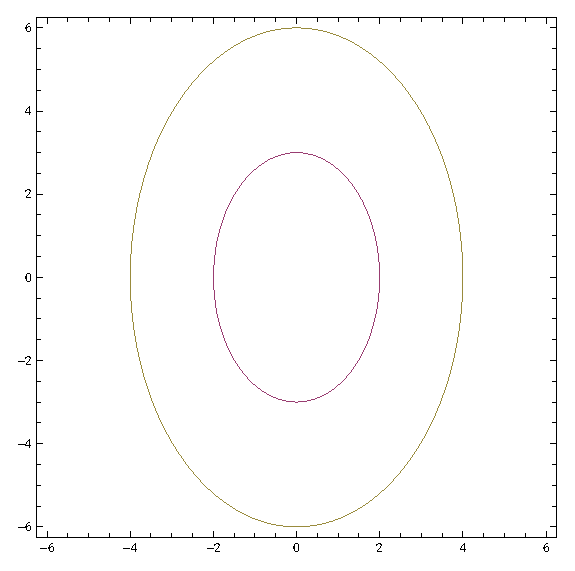
\includegraphics[scale=0.7]{1i.eps} 
\end{minipage}
\item 
\begin{minipage}{0.49\columnwidth}
\begin{lstlisting}
Plot3D[x^2/4 + y^2/9 + 4, 
{x, -6, 6}, {y, -6, 6}]
\end{lstlisting}
\end{minipage}
\begin{minipage}{0.50\columnwidth}
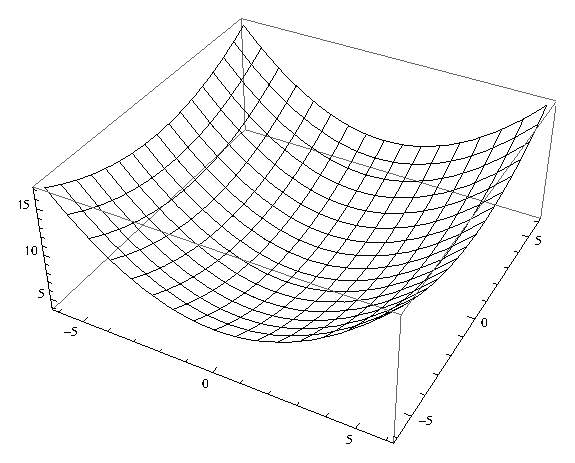
\includegraphics[scale=0.7]{1ii.eps} 
\end{minipage}
\item 
Da $f$ eine Komposition von stetigen Funktionen ist, sowie das Intervall $D$ kompakt ist, muss $f$ Minima und Maxima in $D$ annehmen. Anhand der Bilder ist ein leichtes zu sehen, wo Minima und Maxima auftreten. \textbf{Minima: } $f(0,0) = 4$, \textbf{Maxima: } $f(0,1) = \frac{52}{9}$
\item 
Man kann $\vec{Z}$ nicht zeichnen, da man 4 Dimensionen nicht darstellen kann. Wählt man jedoch $r=1$ sieht das ganze so aus: \\
\begin{minipage}{0.49\columnwidth}
\begin{lstlisting}
Plot3D[{{cos phi}, {sin phi}, {z}}, 
{phi, 0, 6.28}, {z, 0, 2}]
\end{lstlisting}
\end{minipage}
\begin{minipage}{0.50\columnwidth}
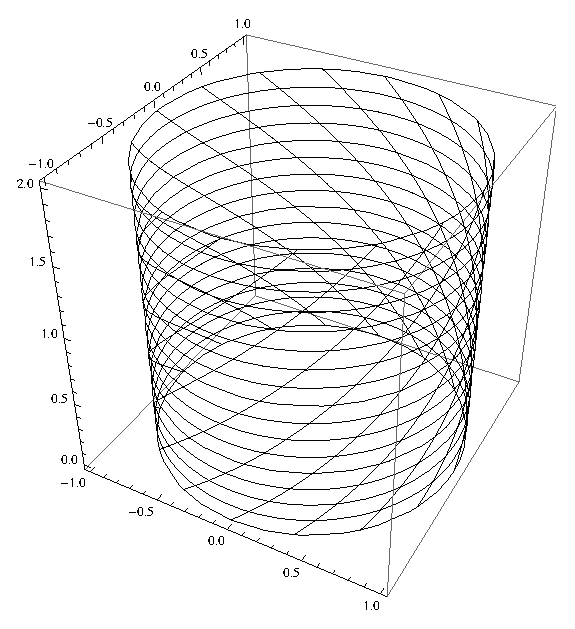
\includegraphics[scale=0.7]{1iv.eps} 
\end{minipage}
\end{enumerate}
\subsection*{Aufgabe 2.}
$f$ ist an den Punkten $(x,y) \neq (0,0)$ stetig da, $\frac{x^2y^2+y^8}{x^2+y^4}$ eine Komposition stetiger Funktionen ist. Sei die Stetigkeit am Punkt $(x,y) = (0,0)$ zu überprüfen.
\begin{align*}
\lim_{\vec{x} \to \vec{0}} \left| f(x,y) - f(0,0) \right| &= \lim_{\vec{x} \to \vec{0}} \left| \frac{x^2y^2+y^8}{x^2+y^4} - 0 \right| \\
 &= \lim_{\vec{x} \to \vec{0}} \left| \frac{x^2y^2+y^8}{x^2+y^4}\right|
\end{align*}
\end{document}
